\documentclass{article}
\usepackage{amsthm} 
\usepackage{physics}
\usepackage{ragged2e}
\usepackage{quoting}
\usepackage{circuitikz}
\usepackage{amsthm}
\usepackage[a4paper, left=1.5cm, right=1.5cm, top=2cm, bottom=2cm]{geometry}
\title{Appunti laboratorio di elettromagnetismo}
\author{ Mirolo Manuele / Alessio Brusini}
\date{a.a. 2025/26}
\newtheorem{theorem}{Teorema}
\begin{document}
\maketitle
\justifying
\tableofcontents
\newpage
\section{Lezione 22/09/2025}
\subsection{Richiami di elettromagnetismo}
\begin{itemize}
    \item La carica elettrica è quantizzata, ovvero esiste una carica elementare $1 e = 1.6 \cdot 10^{-19} C$
    \item Legge di Coulomb, che descrive la forza repulsiva/attrattiva tra due cariche puntiformi:
    \[
    \vec{F}_{1,2} = \frac{Q_1 Q_2}{4\pi\epsilon_0 r^2}
    \]
    dove $\epsilon_0 = 8.85 \cdot 10^{-12} \frac{C^2}{N \cdot m^2}$ è la costante dielettrica del vuoto.
    
    Possiamo notare che il campo elettrico è conservativo, per cui esiste un \textit{potenziale elettrico} $V$: 

    \begin{equation*}
        V=\frac{Q}{4 \pi \epsilon_0 r} \quad \vec{F} = - \vec{\nabla} V 
    \end{equation*}

    \item Definiamo \textbf{corrente elettrica} attraverso una superfice delimitante 2 regioni di spazio, la cui unità di misura è l'Ampere (A), tramite:
    \[
    I = \frac{dQ}{dt}
    \]

    Vale la legge sperimentale detta \textit{1° legge di Ohm}:
    \[
    V = R I
    \]
    dove $R$ è la resistenza del conduttore, che dipende dalla sua natura e dalla sua geometria, da cui la \textit{2° legge di Ohm}:
    \[
    R= \int_{0}^{l} \frac{d\rho(l')}{\Sigma(l')} dl'
    \]
    dove $\rho$ è la resistività del materiale e $\Sigma$ è la sezione del conduttore.
    
    La sua unità di misura è l'Ohm ($\Omega$):
    \[
    1 \Omega = 1 \frac{V}{A}
    \]

    \item La resistività dipende dalla temperatura secondo la legge:
    \[
    \rho(T) = \rho_{20} [1 + \alpha (T - 20^\circ C)]
    \]

    \item Definiamo \textbf{potenza elettrica}, effettuando un lavoro L per spostare una carica fra due punti, come:
    \[
    W = \frac{dL}{dt} = V I = I^2 R = \frac{V^2}{R}
    \]

    \item In un atomo unico il potenziale atomico tende a 0 all'avvicinarsi del nucleo, mentre in un solido la funzione potenziale è periodica a causa della sovrapposizione dei potenziali atomici.
    \item Definiamo \textbf{circuito elettrico} un campo elettrostatico $\vec{F}$ conservativo, il lavoro lungo un percorso chiuso è nullo, introduciamo allora un potenziale U, con dU differenziale esatto.
    
    Se la forza elettrica è originata da una distribuzione di carica \textbf{Q}, definiamo il \textbf{campo elettrico} $\mathbf{\vec{E}(\vec{r})}$ in ogni punto dello spazio. Tale \textbf{Q} permette di spostare una carica di prova \textbf{q} in $\vec{r}$ con una forza $\vec{F_e}(\vec{r}) = q \vec{E}(\vec{r})$

    Si definisce una \textit{funzione differenza di potenziale} $\Delta U = q \Delta $ e $\vec{E}= -\vec{\nabla} V$

        \item In un sistema fisico isolato (es. \textit{maglia conduttrice}), la carica totale si conserva, ovvero $\Delta V_{tot} = 0$, da cui la \textbf{legge di Kirchhoff}:
    \end{itemize}
    
    \begin{theorem}
        La somma delle tensioni ai capi di una maglia è nulla.
    \end{theorem}
    \[
    \sum_{k=1}^{n} V_k = 0
    \]

\section{Lezione 25/09/2025}
A causa di Benjaming Franklin la corrente va dal polo positivo a quello negativo, in quanto si pensava che fossero cariche positive a spostarsi, non quelle \textbf{negative} come avviene nella realtà.
La corrente all'interno di un circuito rimane costante, per la legge della conservazione della carica.
 
Nel momento in cui la corrente incontra un \textit{nodo}, una biforcazione,
trova due vie possibile da percorrere, per la conservazione avremmo:
$I_{tot}= I_1 + I_2$ \\
\begin{center}
\begin{circuitikz}
    % Punto nodale principale
    \draw(0,0) node[circ] (A) {} 
        to[short, label=$I$] (2,0) node[circ, label=above:$N$] (B) {}
        to[short, label=$I_1$] (3,-1) node[circ] (C) {};
    
    % Collegamenti aggiuntivi
    \draw(B) to[short, label=$I_2$] (3,1) node[circ] {};
\end{circuitikz}
\end{center}
Finchè il circuito è un sistema isolato, le correnti prese con i loro segni seguono la seguente legge: 
\[
I_{tot} = \sum_{k=1}^{n} I_k \; \rightarrow \; \sum_{k=1}^{n} I_k-I_{tot}=\sum_{j=1}^{n+1} I_j =0
\]

Da cui la \textbf{2° legge di Kirchhoff}:  \\
\centering
\textit{se un circuito costituisce un sistema isolato, la somma
delle correnti entranti in un suo nodo è uguale alla somma delle correnti uscenti dallo stesso nodo}
\justifying


Queste leggi valgono in \textit{corrente continua}, ovvero quando la corrente non varia nel tempo. 

\begin{itemize}
    \item Definiamo la \textbf{forza elettromotrice} (f.e.m.) come la differenza di potenziale tra i due poli di un generatore, generata da fennomeni chimici quali le reazioni di ossido-riduzione.
In realtà non si tratta di una forza, ma il potenziale elettrico:
\[
V_{1i}= - k \frac{q_1 q_i}{r_{1i}} \rightarrow F_{1i} = - \nabla V_{1i} 
\]
Una d.d.p. può non essere in grado di mantenere una corrente costante, in quanto la resistenza del circuito può variare nel tempo (bastoncino caricato). Ma queste correnti non osccillanti lo possono diventare applicando lavoro.\\
\textbf{N.B} : non sempre un voltaggio di corrente è equivalente alla sua forza elettromotrice.  

\item La f.e.m. garantisce che la corrente scorra nel circuito, in quanto fornisce energia al sistema (che viene persa dagli elettroni che viaggiano nel cirucito e vengono deviati dagli urti). Per quest'ultimo motivo introduciamo la 
\textbf{resistenza} (R). Poichè l'elettrone fa "più fatica" se ci sono meno vie e possibile e se le "porte d'ingresso" sono più strette, si deve avere:
\[
R \propto \frac{l}{\Sigma}
\]
dove $\Sigma$ è l'area della sezione retta del conduttore.

Tramite prove sperimentali si introduce la \textbf{legge di Ohm} (nell'ipotesi di materiale omogeneo e di sezione costante):
\[
R= \rho \frac{l}{\Sigma}
\]
dove $\rho (\theta)$ è la resistività del materiale, che dipende molto da $T$; inoltre $L \propto T$ e $\Sigma \propto T^2$, ma tali effetti si compensano. Da cui:
\[
\rho(\theta) \simeq \rho_{\theta^*}(1 + \alpha (\theta - \theta^*))
\]
dove $\theta^*$ è la temperatura di riferimento, che cambia per ingegneri e fisici (solitamente in rete è $\theta=20^{\circ}$).

Da ciò deriva il fatto che $R \propto T$.

\item Per l'intensità invece avremo 
\[
I = \frac{V}{R} \rightarrow V = R I
\]
Tutte le leggi sono \textit{fenomenologiche}, non derivano da principi primi.
\end{itemize}
La formula più realistica che rappresenta la resistenza di un tratto di circuito è la seguente:
\[
R = \int_{l_1}^{l_2} \frac{\rho(l')}{\Sigma(l')} dl'
\]
ovvero un integrale curvilineo\\

\begin{center}
\begin{circuitikz}
    % Circuito base: pila + resistore
    \draw(0,0) to[battery, l=$V$] (0,2)
          to[short] (2,2)
          to[R, l=$R_1$] (2,0)
          to[R, l=$R_2$] (0,0);
    
          \draw (2,0) node[circ, label=below:$B$] {};
            \draw (0,2) node[circ, label=above:$A$] {};
            \draw (0,0) node[circ, label=below:$C$] {};
\end{circuitikz}
\end{center}
Siccome supponiamo che il circuito sia un sistema isolato, valgono
\[
V_{tot} = V_{AB} + V_{BC} \quad I=VR_{eq} \rightarrow R_{eq} = R_1 + R_2
\]

\section{Lezione 29/09/2025}
\subsection{Resistenze in serie e parallelo}
Vediamo un altro tipo di circuito, che rappresenta un \textbf{partitore di correnti}
\begin{center}
\begin{circuitikz}
  \draw
  (0,0) to[battery, l=$V$] (0,4)
  to[short] (2,4)
  to[R=$R_1$] (2,0)
  (2,4) to[short] (4,4)
  (4,4) to[R=$R_2$] (4,0)
  -- (0,0);
\end{circuitikz}
\end{center}


deve valore la legge di Kirchhoff (sistena isolato) e quella di Ohm:
\[
I=I_1+I_2 
\]
Poichè supponiamo che non ci siano altre resistenze (sistema ideale), la differenza di potenziale ai capi delle due resistenze deve essere la stessa (dalla legge di Ohm):
\[
\frac{V}{R_{eq}} = \frac{V}{R_1} + \frac{V}{R_2} \rightarrow \frac{1}{R_{eq}} = \frac{1}{R_1} + \frac{1}{R_2} = \frac{R_1 + R_2}{R_1R_2}
\]

Supponiamo di avere un solo alimentatore e dover far funzionare tre dispositivi, utilizziamo un \textbf{partitore di tensione}
\begin{center}
\begin{circuitikz}[american]

  \draw
    (0,0) node[left] {$A$} to[battery1,l=$V$] (0,-6) node[left] {$D$};
  \draw
    (0,0) -- (2,0)
      to[R=$R_1$, *-*] (2,-2) node[right] {$B$}
      to[R=$R_2$, *-*] (2,-4) node[right] {$C$}
      to[R=$R_3$, *-*] (2,-6) -- (0,-6);
\end{circuitikz}
\end{center}
ovvero un oggetto che permette di dividere la tensione in più parti, stabili nel tempo.


Chiamiamo \textit{corrente continua}, quella che rimane costante per un perio abbastanza lungo di tempo. 
\pagebreak
\subsection{Strumenti per misurare corrente e tensione}
Uno strumento per misurare delle variabili fisiche dovrebbe sempre dare una risposta \textit{lineare}.
Indichiamo con:
\begin{itemize}
\item $\vec{E}$ il campo elettrico,
\item $\vec{B}$ il campo magnetico,
\item $\vec{F_L}$ la forza di Lorentz:
\end{itemize} 
\[
\vec{F_L} = q \vec{E} + q \vec{v} \times \vec{B}
\]
La forza di Lorentz subita da una carica in un campo elettromagnetico è la somma della forza elettrica e della forza magnetica, l'una moltiplicata per la carica e l'altra per la velocità della carica.

Sono tutte quantità relativisticamente invarianti dunque la formula vale sia per la fisica classica che per quella relativistica.

Consideriamo ora il caso di una calamita con i poli avvicinati e presente uno spazio cilindrico tra di loro. Se inseriamo li un segmento cilindrico di ferro dolce (materiale che reagisce velocemente al campo magnetico in cui si trova), allora posso trovare dei segmentini di linee di campo (che ricordiamo essere
ortogonali alla superfice equipotenziale della calamita) 

\begin{center}
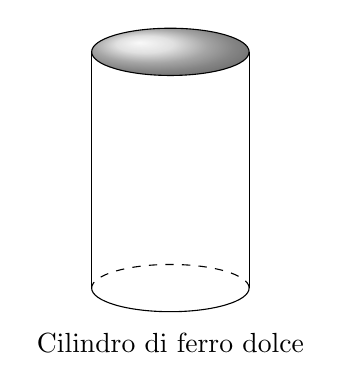
\begin{tikzpicture}
    
% Cilindro (vista 3D semplificata)
\shade[ball color=gray!40, opacity=0.8] (0,0) ellipse (1 and 0.3); % parte superiore
\draw (0,0) ellipse (1 and 0.3); % bordo superiore

\draw (-1,0) -- (-1,-3); % lato sinistro
\draw (1,0) -- (1,-3);   % lato destro

\draw (-1,-3) arc[start angle=180, end angle=360, x radius=1, y radius=0.3]; % base visibile
\draw[dashed] (1,-3) arc[start angle=0, end angle=180, x radius=1, y radius=0.3]; % base nascosta

% Etichetta
\node at (0,-3.7) {Cilindro di ferro dolce};

\end{tikzpicture}
\end{center}

Se supponiamo di avvolgere tale cilindro con una spira e facciamo passare corrente elettrica, chiamati a e b i lati corto e lungo della spira e 
osservando il più classico degli \textit{elettroni di conduzione} con velocità $v$, il tratto di spira a sarà ortogonale al campo magnetico 
\[
e^- v \times B = e^- v B 
\]
L'elettrone viene "spinto fuori dalla spira"

Contrariamente nel tratto b, l'elettrone non viene deviato, in quanto la velocità è parallela a $B$. Tornato nel tratto A, se I rimane costante avremo nuovamente $\vec{F_L}$, sempre diretta verso l'esterno.

Questa coppia di forze genera un \textit{momento torcente} pari a: $\tau = e^- v B b $

Il flusso invece è dato dalla \textit{densità dei portatori di carica} $\lambda$, dunque scrivendo la corrente come $ v A \lambda e =I = \frac{dq}{dt}$, da cui
\[
\tau = B I b = B n a b I \quad I = \lambda a e v 
\]

Bilanciamo questo momento con una forza elastica grazie a delle molle elicoidali controrotanti (in modo da bilanciare le imperfezioni), ricordando che (nell'approsimazione di $\theta < 4^\circ$):
\[
\tau_{el} \approx k \theta = \tau_{mag} = B I b \rightarrow \theta = \frac{B n a b}{k} I
\]
Dobbiamo dunque risaltare il nostro segnale, per questo la molla ha più spire (non più di 10 per evitare deformazioni), in tal modo inoltre, l'approsimazione angolare vale fino a $\theta < 40^\circ$ (max $\theta = 3600^\circ$).

Nel caso della realtà abbiamo il cosidetto \textit{effetto Joule}, ovvero il riscaldamento del conduttore, quindi posso usare solo piccole correnti 
Lo strumento appena descritto è detto \textbf{Amperometro}, costruendo un circuito con una resistenza e un amperometro in parallelo, possiamo misurare la corrente che passa nel circuito.
avremmo
\[
I= I_A + I_S= \frac{V}{R_A}+ \frac{V}{R_S}
\]
costruiamo la resistenza in modo che $R_A << R_S$ (per esempio $\frac{R_A}{R_S}=\frac{1}{10}$), tali $R_S$ sono dette \textbf{resistenze di shunt}. La precisione, dunque, diminuisce in modo direttamente proporzianale all'aumento del numero di resistenze 













\end{document}